\documentclass[10pt]{beamer}
\usetheme{jambro}

\title[]{Pensamento Econômico Contemporâneo - A escola Keynesiana ortodoxa}
\author[]{Paulo Victor da Fonseca}
\date{}

\hypersetup{
    colorlinks = true,
    urlcolor = teal,
    linkcolor = teal    
}
\usepackage[portuguese]{babel}
\usepackage{subfig}
\usepackage{emoji}

\begin{document}

\begin{frame}[plain]
    \titlepage{
        \begin{center}
            \begin{minipage}{0.8\textwidth}
                \centering
            \end{minipage}
        \end{center}}
\end{frame}

\begin{frame}{Sumário}
    \tableofcontents
\end{frame}

\section{Introdução}
\begin{frame}{Introdução}
    \begin{itemize}
        \item Samuelson ($\approx$ 1950) e a \textcolor{blue}{síntese neoclássica}: amplamente aceito que a micro neoclássica e a macro Keynesiana poderiam `conviver'
        \bigskip
        \item O modelo clássico/neoclássico permaneceu relevante para questões micro e análise de crescimento de longo prazo
        \bigskip
        \item A macro Keynesiana ortodoxa fornecia a abordagem mais útil de análise de fenômenos agregados de curto prazo
        \bigskip
        \item Esta nova visão foi o paradigma macroeconômico dominante até meados dos anos 1970s
    \end{itemize}
\end{frame}

\begin{frame}{Introdução}
    \begin{itemize}
        \item Nossos objetivos nesta nova seção da disciplina podem ser, assim, sumarizados:
        \bigskip
        \begin{enumerate}
            \item Revisar a interpretação ortodoxa da teoria Keynesiana - modelo IS-LM - para uma economia fechada
            \medskip
            \item Discutir a análise original da curva de Phillips e sua importância para a análise Keynesiana ortodoxa
            \medskip
            \item Resumir as principais proposições da economia Keynesiana ortodoxa
        \end{enumerate}
    \end{itemize}
\end{frame}

\begin{frame}{Introdução}
    \begin{itemize}
        \item Ao longo deste bloco, duas questões recorrentes e interrelacionadas irão emergir:
        \bigskip
        \begin{enumerate}
            \item A controvérsia acerca das propriedades auto-equilibradoras do sistema econômico
            \medskip
            \item O papel de políticas governamentais intervencionistas
        \end{enumerate}
    \end{itemize}
\end{frame}

\begin{frame}{Introdução}
    \begin{itemize}
        \item Características/crenças definidoras da escola Keynesiana ortodoxa:
        \bigskip
        \begin{enumerate}
            \item \textcolor{purple}{A economia é inerentemente estável e sujeita a choques erráticos}. Estes choques são atribuídos, principalmente, a variações na eficiência marginal do investimento devido a mudanças no estado de confiança dos empresários - `animal spirits'
            \medskip
            \item \textcolor{purple}{Se deixada aos seus próprios mecanismos, a economia pode levar um longo tempo para retornar ao equilíbrio de pleno emprego após ser sujeita a algum choque}
            \medskip
            \item \textcolor{purple}{Nível agregado de produto e emprego essencialmente determinados pela DA e formuladores de política podem influenciar o nível de demanda agregada `efetiva' para assegurar uma convergência mais rápida ao pleno emprego}
            \medskip
            \item \textcolor{purple}{Em termos de política de estabilização, a política fiscal é geralmente preferível à política monetária}. Dado que os efeitos de medidas de política fiscal são consideradas mais diretas, previsíveis e mais ágeis em influenciar a DA
        \end{enumerate}
    \end{itemize}
\end{frame}

\section{Modelo IS-LM: economia fechada}
\subsection{Introdução}
\begin{frame}{Introdução}
    \begin{itemize}
        \item Origem do modelo Keynesiano ortodoxo: `Mr. Keynes and the Classics: A suggested interpretation' de John Hicks (1937)
        \bigskip
        \item Modelo Hicksiano aperfeiçoado por Modigliani (1944) e popularizado nos EUA por Hansen (1949, 1953)
        \bigskip
        \item Por quase meio século, o modelo IS-LM Hicksiano tornou-se no modelo estabelecido para desenvolvimento de teorias macro e teve enorme influência nas direções de políticas macro até meados dos anos 1960s
    \end{itemize}
\end{frame}

\subsection{O mercado de bens e serviços e a curva IS}
\begin{frame}{O mercado de bens e serviços e a curva IS}
    \begin{itemize}
        \item Equilíbrio no mercado de bens e serviços ocorre quando DA se iguala à oferta agregada de bens
        \bigskip
        \item No modelo Keynesiano ortodoxo, assume-se que o nível de produto e emprego é determinado inteiramente pela DA
        \bigskip
        \item Em uma economia fechada, a demanda agregada é composta por consumo, investimento e gastos públicos
        \bigskip
        \item Assume-se que os gastos com consumo dependem positivamente da renda disponível
        \bigskip
        \item Gastos do governo exogenamente determinados
        \bigskip
        \item O nível de investimento é uma função negativamente relacionada à taxa de juros - uma variável determinada endogenamente pelas interações entre os mercados de bens e financeiros
    \end{itemize}
\end{frame}

\begin{frame}{O mercado de bens e serviços e a curva IS}
    \begin{itemize}
        \item A \hlight{curva IS} define um locus de combinações entre taxas de juros e renda que estão associados com o equilíbrio no mercado de bens
        \bigskip
        \item O nome deriva da condição de equilíbrio que, em uma economia fechada sem setor público, o nível de investimento ($I$) se iguala ao nível de poupança ($S$)
        \bigskip
        \item Dada a hipótese de uma função investimento negativamente relacionada com a taxa de juros, a curva IS é negativamente inclinada
        \bigskip
        \item \emph{Ceteris paribus}, à medida que a taxa de juros declina, o nível de investimento aumenta, resultando em um aumento do nível de produto agregado
    \end{itemize}
\end{frame}

\begin{frame}{O mercado de bens e serviços e a curva IS}
    \begin{itemize}
        \item A inclinação da curva IS depende da elasticidade-juros da função investimento e do valor do multiplicador Keynesiano
        \bigskip
        \item A curva IS será \textcolor{blue}{mais} (\textcolor{red}{menos}) inclinada quanto \textcolor{blue}{menor} (\textcolor{red}{maior}) for a resposta do investimento a variações na taxa de juros e quanto \textcolor{blue}{menor} (\textcolor{red}{maior}) for o valor de multiplicador
        \bigskip
        \item E.g., \emph{ceteris paribus}, quanto menos o investimento aumenta à medida que a taxa de juros diminui, menos a renda agregada aumentará, gerando uma curva IS mais inclinada
        \bigskip
        \item De maneira similar, quanto menor o valor do multiplicador, menos a renda agregada aumentará seguindo um aumento do nível de investimentos e, portanto, mais inclinada será a curva IS
        \bigskip
        \item No caso extremo (extremamente Keynesiano) em que o investimento é perfeitamente inelástico, a curva IS será vertical
    \end{itemize}
\end{frame}

\begin{frame}{O mercado de bens e serviços e a curva IS}
    \begin{itemize}
        \item É importante ressaltar que a IS curva é obtida para um dado nível de gastos do governo, de tributação e expectativas, de forma que uma política fiscal expansionista desloca a curva IS para a direita
        \bigskip
        \item E.g., um aumento nos gastos do governo está associado com um nível mais elevado de renda agregada para qualquer nível de taxa de juros, de forma que o deslocamento para a direita da curva IS é igual ao produto entre o aumento nos gastos do governo e o valor do multiplicador Keynesiano
    \end{itemize}
\end{frame}

\subsection{O mercado monetário e a curva LM}
\begin{frame}{O mercado monetário e a curva LM}
    \begin{itemize}
        \item O equilíbrio no mercado monetário ocorre quando a oferta e a demanda por moeda se equalizam
        \bigskip
        \item Assume-se que a oferta de moeda é determinada exogenamente pela autoridade monetária
        \bigskip
        \item Dentro do modelo Keynesiano, há três principais motivos para que os indivíduos retenham moeda em seus portfólios:
        \bigskip
        \begin{enumerate}
            \item Motivo transação
            \medskip
            \item Motivo precaução
            \medskip
            \item Motivo especulação
        \end{enumerate}
    \end{itemize}
\end{frame}

\begin{frame}{O mercado monetário e a curva LM}
    \begin{itemize}
        \item A demanda por encaixes reais por motivos transação e precaução variam positivamente com a renda
        \bigskip
        \item A demanda por motivo especulação depende do nível atual de taxa de juros relativamente à taxa de juros `normal'
        \bigskip
        \item Ao assumir que pessoas diferentes possuem expectativas distintas acerca da trajetória futura da taxa de juros, é possível postular uma demanda por moeda que varie inversamente com a taxa de juros
        \bigskip
        \item Quanto mais alta a taxa de juros atual (relativamente ao nível considerado normal), maior o número de indivíduos que esperam reduções futuras na taxa de juros (e, consequentemente, uma trajetória ascendente nos preços dos títulos) e, portanto, menor será a demanda por moeda por motivo especulação
    \end{itemize}
\end{frame}

\begin{frame}{O mercado monetário e a curva LM}
    \begin{figure}
        \centering
        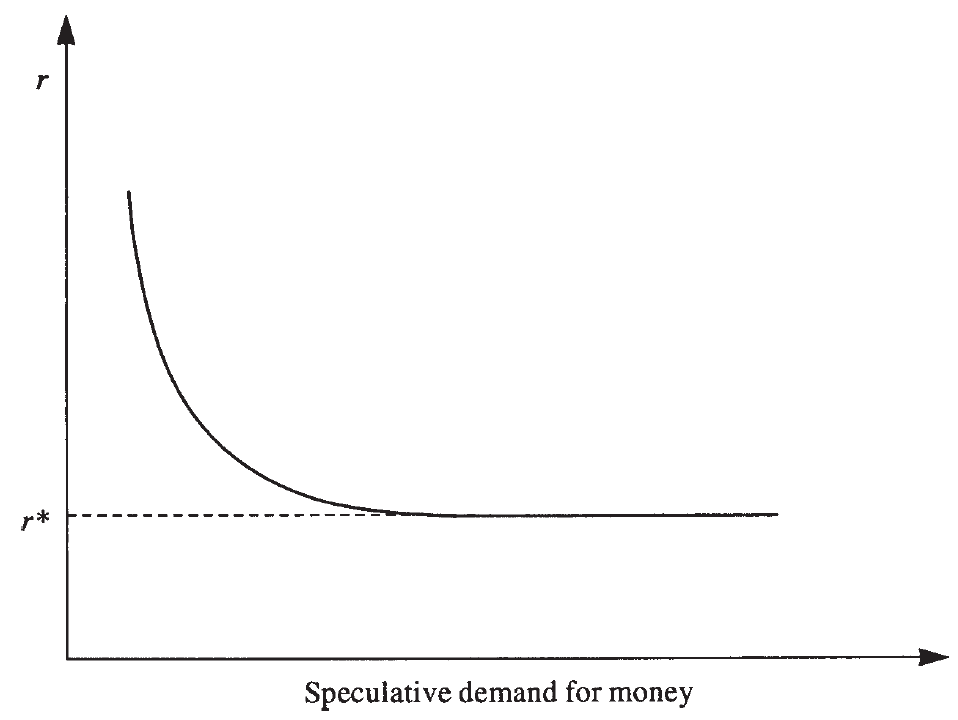
\includegraphics[width=0.6\textwidth]{./figures/aula06_fig1.PNG}
        \caption{Demanda especulativa por moeda. Fonte: Snowdon e Vane (2005).}
        \label{fig1}
    \end{figure}
\end{frame}

\begin{frame}{O mercado monetário e a curva LM}
    \begin{itemize}
        \item A possibilidade teórica de que, a níveis muito baixos de taxas de juros (que espera-se que prevaleça em um caso de equilíbrio de subemprego), a demanda por moeda pode tornar-se perfeitamente elástica com relação à taxa de juros
        \bigskip
        \item Este fenômeno é ilustrado pela Figura \ref{fig1} em sua seção horizontal no nível $r^*$
        \bigskip
        \item Em $r^*$ as expectativas dos agentes convergem, dado que todos os indivíduos esperam que a única trajetória possível para a taxa de juros seja ascendente e, portanto, a demanda por moeda se torna perfeitamente elástica com relação aos juros: \textcolor{blue}{armadilha da liquidez}
    \end{itemize}
\end{frame}

\begin{frame}{O mercado monetário e a curva LM}
    \begin{itemize}
        \item Com relação à armadilha da liquidez, cabe ressaltar que Keynes a enunciou apenas como uma possibilidade teórica e até comentou que não tinha ciência de que poderia ocorrer na prática
        \bigskip
        \item No entanto, como veremos mais adiante, este fenômeno tornou-se particularmente importante para a análise de equilíbrio de subemprego no modelo Keynesiano ortodoxo
        \bigskip
        \item Além disso, hoje já temos evidências empíricas de países que experienciaram situações de armadilha da liquidez
    \end{itemize}
\end{frame}

\begin{frame}{O mercado monetário e a curva LM}
    \begin{itemize}
        \item A \hlight{curva LM} define um locus de combinações entre taxas de juros e renda que estão associadas com o equilíbrio no mercado monetário
        \bigskip
        \item O nome deriva da condição de equilíbrio no mercado monetário onde a demanda por moeda, ou como Keynes denominou - preferência pela liquidez (L) - se iguala à oferta de moeda (M)
        \bigskip
        \item Dadas as hipóteses de que a demanda por moeda é positivamente relacionada com a renda e negativamente inclinada com a taxa de juros, a curva LM é positivamente inclinada
    \end{itemize}
\end{frame}

\begin{frame}{O mercado monetário e a curva LM}
    \begin{itemize}
        \item \emph{Ceteris paribus}, à medida que a renda aumenta, a demanda transacional e precaucional por moeda aumenta o que, dada uma oferta de moeda, demanda um aumento na taxa de juros para reduzir a demanda especulativa por moeda e manter o equilíbrio no mercado monetário
        \bigskip
        \item A inclinação da curva LM depende da elasticidade-renda e da elasticidade-juros da demanda por moeda
        \bigskip
        \item A curva LM será \textcolor{blue}{mais} (\textcolor{red}{menos}) inclinada quanto \textcolor{blue}{maior} (\textcolor{red}{menor}) for a elasticidade-renda e quanto \textcolor{blue}{menor} (\textcolor{red}{maior}) for a elasticidade-juros da demanda por moeda
    \end{itemize}
\end{frame}

\begin{frame}{O mercado monetário e a curva LM}
    \begin{itemize}
        \item E.g., \emph{ceteris paribus}, quanto mais a demanda por moeda aumentar seguindo um aumento na renda, maior será o aumento na taxa de juros necessário para manter o equilíbrio no mercado monetário, gerando uma curva LM mais inclinada
        \bigskip
        \item Temos, então, dois casos limites:
        \bigskip
        \begin{enumerate}
            \item \textcolor{blue}{Caso clássico}: a demanda por moeda é perfeitamente inelástica com relação à taxa de juros (curva LM vertical)
            \medskip
            \item \textcolor{blue}{Armadilha da liquidez}: a demanda por moeda é perfeitamente elástica com relação à taxa de juros (curva LM horizontal)
        \end{enumerate}
    \end{itemize}
\end{frame}

\begin{frame}{O mercado monetário e a curva LM}
    \begin{itemize}
        \item Curva LM é obtida para valores predeterminados da oferta de moeda, nível de preços e expectativas dos agentes
        \bigskip
        \item De modo que uma expansão monetária desloca a curva LM para a direita
        \bigskip
        \item Seguindo um aumento na oferta de moeda, e uma dada elasticidade-renda da demanda por moeda, qualquer nível de renda deve estar associado a uma taxa de juros mais baixa para preservar o equilíbrio no mercado monetário
        \bigskip
        \item A magnitude do deslocamento depende da elasticidade-juros da demanda por moeda
        \bigskip
        \item Um aumento na demanda por moeda levará a um deslocamento maior (menor) da curva LM quando a demanda por moeda é relativamente elástica (inelástica) com relação à taxa de juros, quando o equilíbrio no mercado monetário é restaurado com uma pequena (grande) queda na taxa de juros
    \end{itemize}
\end{frame}

\subsection{Modelo IS-LM e políticas macroeconômicas}
\begin{frame}{Modelo IS-LM}
    \begin{figure}
        \centering
        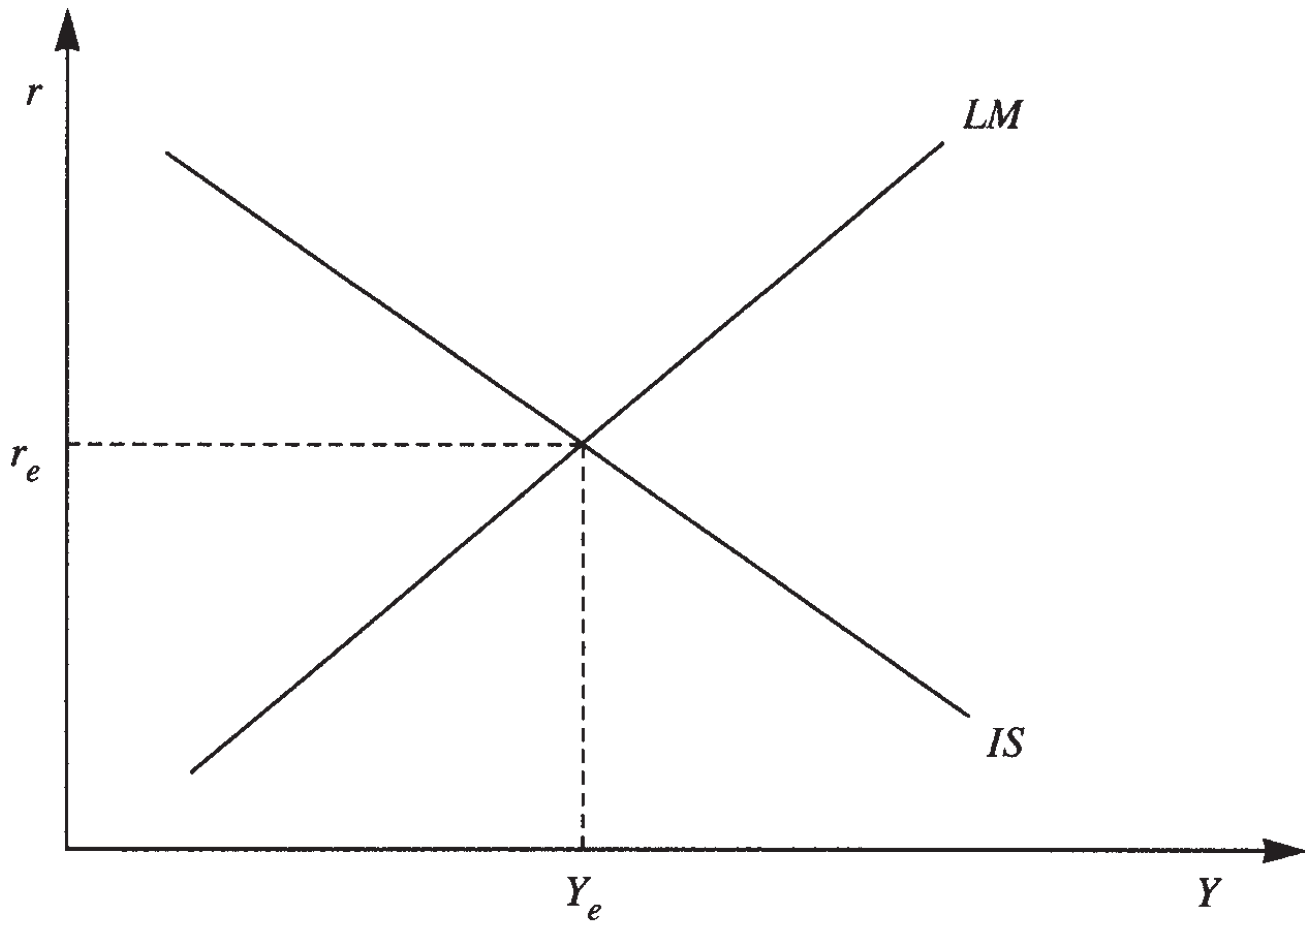
\includegraphics[width=0.6\textwidth]{./figures/aula06_fig2.PNG}
        \caption{O modelo IS-LM generalizado. Fonte: Snowdon e Vane (2005).}
        \label{fig2}
    \end{figure}
\end{frame}

\begin{frame}{Modelo IS-LM completo}
    \begin{itemize}
        \item O equilíbrio nos mercados de bens e monetário é obtido simultaneamente no ponto de intersecção entre as curvas IS e LM - $r_eY_e$ na Figura \ref{fig2}
        \bigskip
        \item Dois pontos devem ser observados:
        \bigskip
        \begin{enumerate}
        \item A intersecção entre as curvas representa o \textcolor{blue}{único} valor de combinação de taxa de juros e renda consistente com o equilíbrio em ambos os mercados
        \medskip
        \item Se o nível de renda está abaixo do nível de pleno emprego, então, tanto a política fiscal quanto monetária podem ter um papel importante em estabilizar a economia
        \end{enumerate}
    \end{itemize}
\end{frame}

\begin{frame}{Eficácia da política fiscal}
    \begin{figure}
        \centering
        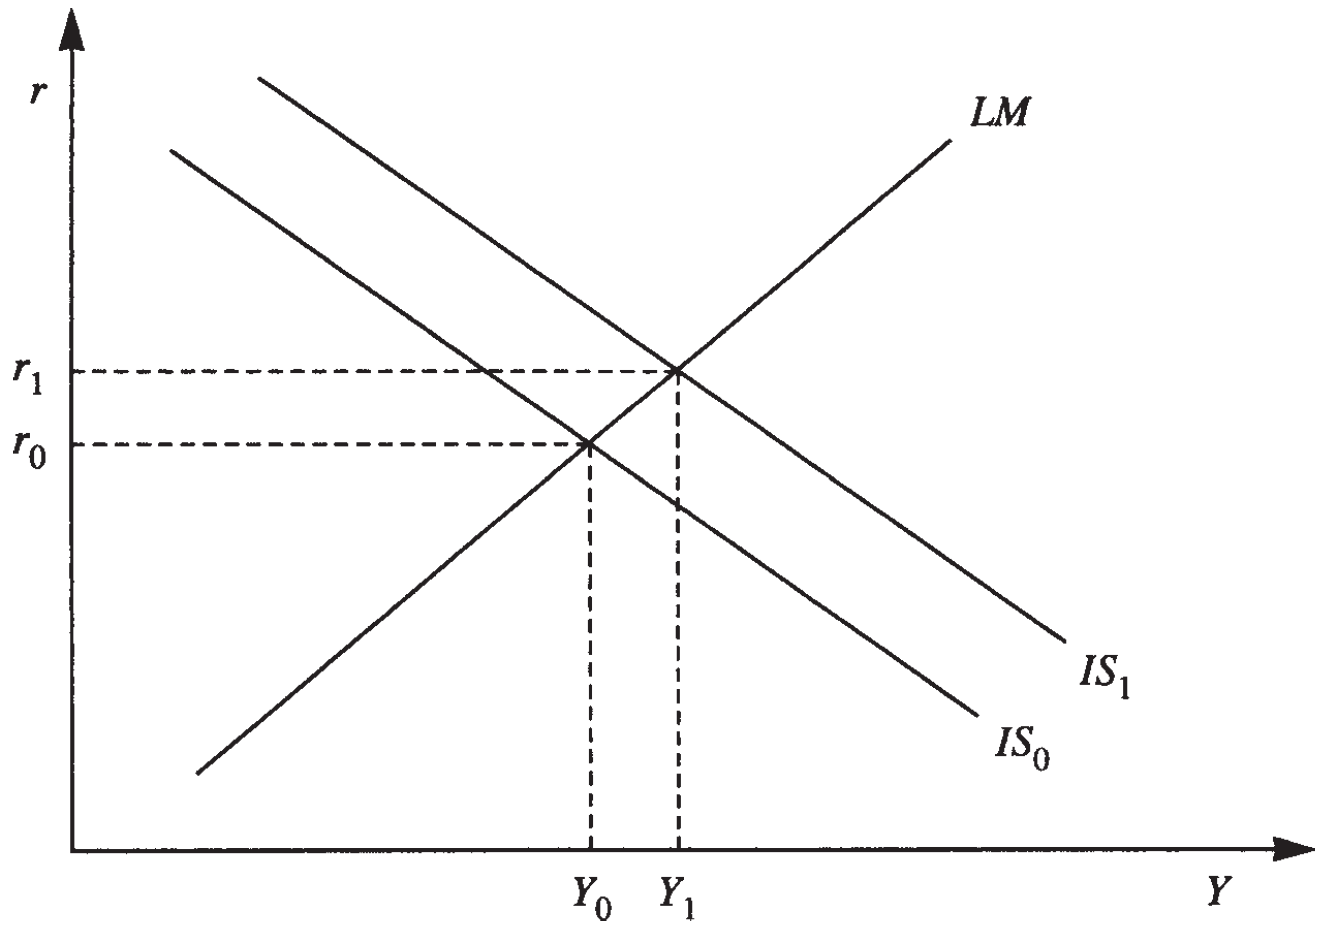
\includegraphics[width=0.6\textwidth]{./figures/aula06_fig3.PNG}
        \caption{Política fiscal expansionista. Fonte: Snowdon e Vane (2005).}
        \label{fig3}
    \end{figure}
\end{frame}

\begin{frame}{Eficácia da política fiscal}
    \begin{itemize}
        \item Uma política fiscal expansionista desloca a curva IS para a direita e resulta em um aumento tanto da taxa de juros de equilíbrio quanto do nível de produto agregado
        \bigskip
        \item À medida que os gastos e a renda aumentam, a demanda por moeda por motivos transação e precaução também aumentam
        \bigskip
        \item Com uma oferta monetária fixa, a taxa de juros se eleva
        \bigskip
        \item O aumento na taxa de juros induz uma queda no nível de investimento privado
        \bigskip
        \item A magnitude dessa redução nos investimentos depende da elasticidade-juros do investimento
    \end{itemize}
\end{frame}

\begin{frame}{Eficácia da política fiscal}
    \begin{itemize}
        \item A política fiscal será mais efetiva em influenciar a demanda agregada e, consequentemente, os níveis de produto e emprego:
        \bigskip
        \begin{enumerate}
            \item Quanto mais elástica for a demanda por moeda com relação à taxa de juros (LM menos inclinada)
            \medskip
            \item Quanto menor a elasticidade-juros dos gastos privados com investimento (IS mais inclinada)
        \end{enumerate}
        \bigskip
        \item Temos, ainda, os seguintes casos limites:
        \bigskip
        \begin{enumerate}
            \item \textcolor{blue}{Caso clássico}: curva LM vertical. Neste caso, uma expansão fiscal não tem efeito nenhum sobre o nível de renda, dado que o aumento na taxa de juros irá reduzir o investimento privado em uma magnitude idêntica ao aumento nos gastos públicos. Isto é, temos um efeito crowding-out completo - Visão do Tesouro
            \medskip
            \item \textcolor{blue}{Armadilha da liquidez}: curva LM horizontal. Uma política fiscal expansionista resultará em um efeito multiplicador completo do modelo Keynesiano simples da cruz Keynesiana
        \end{enumerate}
    \end{itemize}
\end{frame}

\begin{frame}{Eficácia da política monetária}
    \begin{figure}
        \centering
        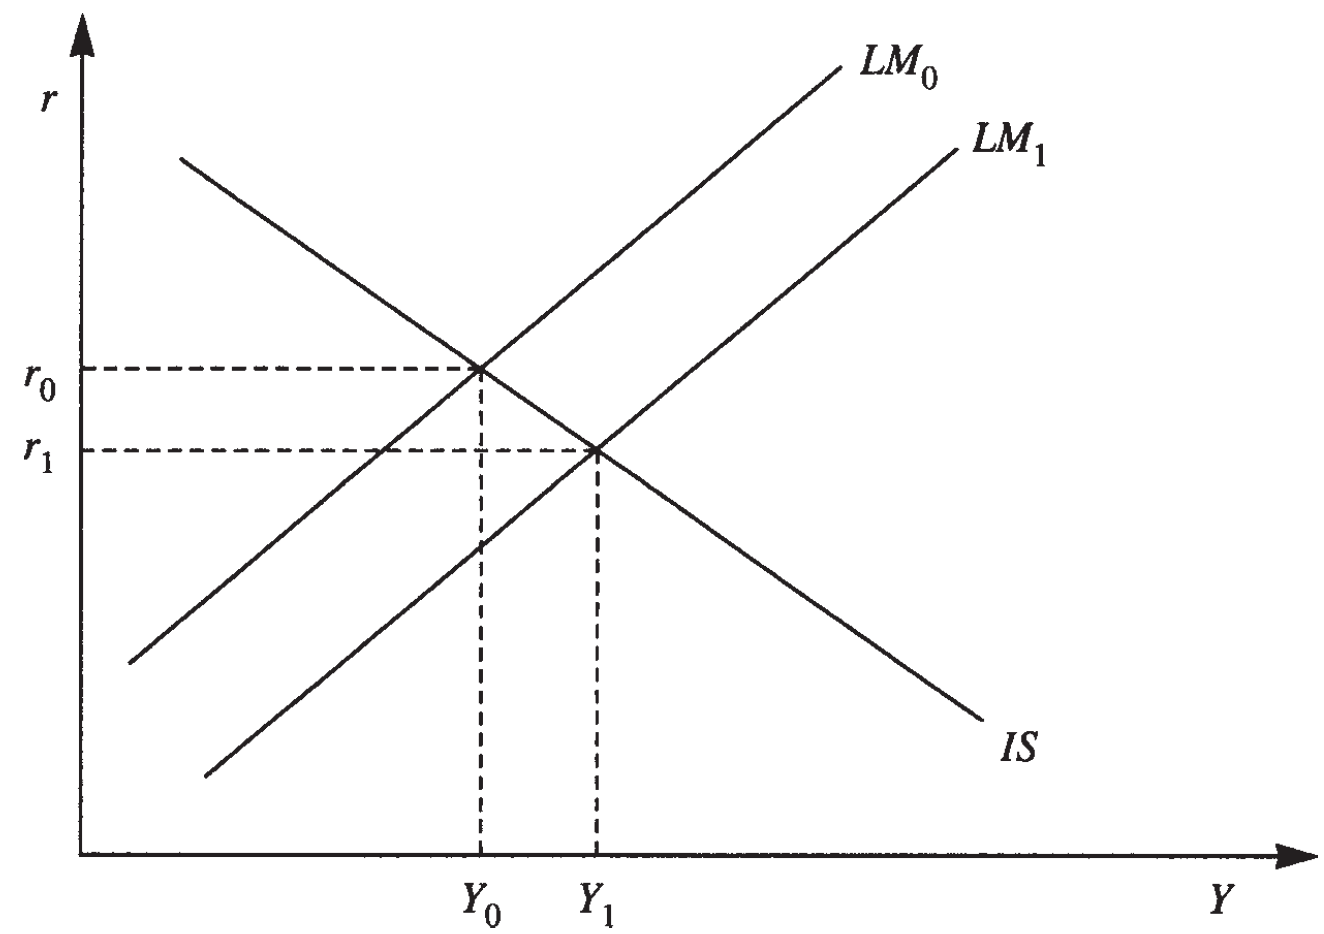
\includegraphics[width=0.6\textwidth]{./figures/aula06_fig4.PNG}
        \caption{Política monetária expansionsita. Fonte: Snowdon e Vane (2005).}
        \label{fig4}
    \end{figure}
\end{frame}

\begin{frame}{Eficácia da política monetária}
    \begin{itemize}
        \item Em uma economia inicialmente em equilíbrio abaixo do pleno emprego, uma política monetária expansionista desloca a curva LM para a direita
        \bigskip
        \item A expansão monetária resulta em uma queda na taxa de juros de equilíbrio e um aumento no nível de renda agregada
        \bigskip
        \item No mecanismo de transmissão da ortodoxia Keynesiana, a força da política monetária depende:
        \bigskip
        \begin{enumerate}
            \item Do grau ao qual a taxa de juros é reduzida seguindo um aumento na oferta monetária
            \medskip
            \item O grau com que o investimento responde a variações na taxa de juros
            \medskip
            \item Do tamanho do multiplicador
        \end{enumerate}
    \end{itemize}
\end{frame}

\begin{frame}{Eficácia da política monetária}
    \begin{itemize}
        \item A eficácia da política monetária em influenciar a DA e, consequentemente, os níveis de produto e emprego é maior:
        \bigskip
        \begin{enumerate}
            \item Quanto mais inelástica com relação à taxa de juros for a demanda por moeda (LM mais inclinada)
            \medskip
            \item Quanto maior a elasticidade-juros do gasto privado com investimento (IS menos inclinada)
        \end{enumerate}
        \bigskip
        \item Nos casos limites de \textcolor{blue}{armadilha da liquidez} (LM horizontal) ou \textcolor{blue}{investimento completamente inelástico com relação aos juros} (IS vertical) o mecanismo de transmissão é rompido e, portanto, a política monetária não terá efeito sobre o nível de produto agregado
    \end{itemize}
\end{frame}

\begin{frame}{Eficácia relativa de políticas macroeconômicas}
    \begin{itemize}
        \item Da discussão anterior fica claro que, embora as políticas fiscal e monetária podem, em situações normais, ser usadas para influenciar o nível de produto e emprego agregados, \textcolor{blue}{a eficácia relativa destes dois instrumentos de política depende dos parâmetros estruturais do modelo, i.e., das inclinações das curvas IS e LM}
        \bigskip
        \item A ortodoxia Keynesiana é, normalmente, caracterizada pelas seguintes observações:
        \bigskip
        \begin{enumerate}
            \item A demanda por moeda é altamente responsiva a variações na taxa de juros (LM relativamente plana)
            \medskip
            \item Investimento é pouco sensível a variações nos juros (IS relativamente mais inclinada)
        \end{enumerate}
    \end{itemize}
\end{frame}

\begin{frame}{Eficácia relativa de políticas macroeconômicas}
    \begin{itemize}
        \item De fato, havia evidências empíricas para a visão ortodoxa Keynesiana associada às elasticidades das curvas IS e LM
        \bigskip
        \item Lawrence Klein, em 1968, afirmou que essa era uma `base empírica sólida'
        \bigskip
        \item Base que, como veremos mais adiante na disciplina, tornou-se cada vez mais questionável durante os anos 1960s
    \end{itemize}
\end{frame}

\begin{frame}{Eficácia relativa de políticas macroeconômicas}
    \begin{itemize}
        \item Nestas circunstâncias (curva IS relativamente mais inclinada e LM mais plana), distúrbios oriundos do lado real da economia (ou seja, deslocamentos estocásticos na curva IS) tendem a dominar as variações na renda agregada
        \bigskip
        \item Portanto, a política fiscal é geralmente preferível dado que é relativamente mais eficaz que a política monetária (relativamente mais fraca)
        \bigskip
        \item Esta análise pode ser vista em termos algébricos
    \end{itemize}
\end{frame}

\begin{frame}{Eficácia relativa de políticas macroeconômicas}
    \begin{itemize}
        \item Começamos assumindo que o nível de preços é fixo quando a economia encontra-se em uma condição de equilíbrio abaixo do nível de pleno emprego
        \bigskip
        \item O dispêndio agregado real ($E$) é igual a um componente de gasto autônomo ($A$), um componente dependente da renda agregada real ($cY$) e um componente que é sensível à taxa de juros ($ar$):
        \begin{equation}
            E = A + cY - ar.
            \label{eq1}
        \end{equation}
        \bigskip
        \item O equilíbrio no mercado de bens ocorre quando a demanda agregada se iguala à oferta agregada de bens:
        \begin{equation}
            E = Y.
            \label{eq2}
        \end{equation}
    \end{itemize}
\end{frame}

\begin{frame}{Eficácia relativa de políticas macroeconômicas}
    \begin{itemize}
        \item Nos mercados monetários, a demanda por encaixes reais ($M/P$) tem um componente dependente da renda real ($mY$) e um componente sensível à taxa de juros ($br$):
        \begin{equation}
            \frac{M}{P} = mY - br.
            \label{eq3}
        \end{equation}
        \bigskip
        \item Assume-se que a oferta nominal de moeda é determinada exogenamente pela autoridade monetária ($\bar{M_s}$)
        \bigskip
        \item O equilíbrio no mercado monetário ocorre quando a demanda por moeda iguala-se à oferta:
        \begin{equation}
            \frac{M}{P} = \frac{\bar{M_s}}{P}.
            \label{eq4}
        \end{equation}
    \end{itemize}
\end{frame}

\begin{frame}{Eficácia relativa de políticas macroeconômicas}
    \begin{itemize}
        \item Portanto, a equação em forma reduzida para o nível agregado de renda real é dada por:
        \begin{equation}
            Y = \frac{1}{1 - \left(c - \frac{a}{b}m \right)}A + \frac{1}{m + \frac{b}{a}(1-c)} \frac{\bar{M_s}}{P}.
            \label{eq5}
        \end{equation}
        \bigskip
        \item Como vimos, nesta abordagem, Keynesianos ortodoxos podem ser caracterizados como indivíduos com baixos valores de $a$ e altos valores de $b$
        \bigskip
        \item Portanto, a equação (\ref{eq5}) evidencia que quando a fração $a/b$ é pequena:
        \bigskip
        \begin{enumerate}
            \item Distúrbios do lado real da economia tendem a dominar as variações na renda
            \medskip
            \item A política fiscal é, relativamente, mais forte com o multiplicador de gastos autônomos tendendo a $1/(1-c)$
            \bigskip
            \item A política monetária é, relativamente, mais fraca com o multiplicador monetária tendendo a zero
        \end{enumerate}
    \end{itemize}
\end{frame}

\begin{frame}{Críticas à eficácia relativa da política fiscal}
    \begin{itemize}
        \item A crença dos Keynesianos ortodoxos na efetividade relativa da política fiscal foi questionada, entre outros, pelos monetaristas
        \bigskip
        \item Monetaristas argumentam que, no longo prazo, uma expansão fiscal `pura' (isto é, expansão sem que haja uma acomodação na oferta monetária) resultará em um efeito crowding-out (deslocamento) ou uma substituição dos componentes de gastos privados com efeitos relativamente menores na demanda agregada, níveis de renda e emprego
        \bigskip
        \item Várias razões para a existência de um efeito crowding-out no modelo IS-LM foram dadas que não estão relacionadas com a demanda por moeda sendo perfeitamente inelástica com relação aos juros (LM vertical): e.g., \textcolor{blue}{expectativas dos agentes e efeitos-renda}
    \end{itemize}
\end{frame}

\subsection{Modelo IS-LM estendido: a restrição orçamentária do governo}
\begin{frame}{Modelo IS-LM estendido}
    \begin{itemize}
        \item Na presente análise discutiremos a contra-argumentação dos Keynesianos ortodoxos para reafirmar a importância da política fiscal
        \bigskip
        \item Focaremos nos efeitos renda gerados por uma política fiscal expansionista financiada por emissão de títulos públicos
        \bigskip
        \item Esta análise envolve uma versão estendida do modelo IS-LM, incorporando a restrição orçamentária do governo
    \end{itemize}
\end{frame}

\begin{frame}{Modelo IS-LM estendido}
    \begin{figure}
        \centering
        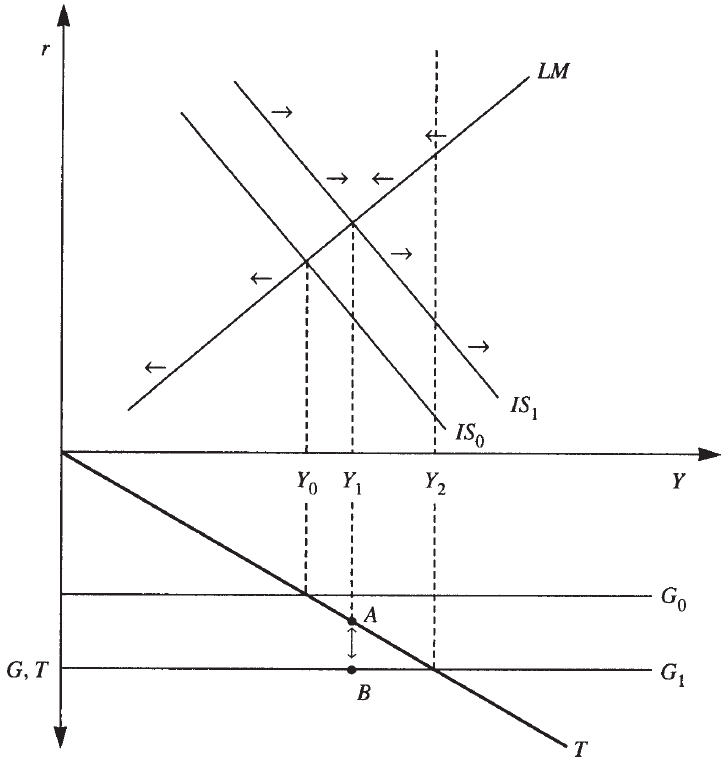
\includegraphics[width=0.4\textwidth]{./figures/aula06_fig5.PNG}
        \caption{Restrição orçamentária do governo e expansão fiscal financiada por títulos. Fonte: Snowdon e Vane (2005).}
        \label{fig5}
    \end{figure}
\end{frame}

\begin{frame}{Modelo IS-LM estendido}
    \begin{itemize}
        \item O painel superior da Figura \ref{fig5} ilustra o modelo IS-LM convencional
        \bigskip
        \item O painel inferior representa a posição orçamentária do governo, determinada pela relação entre gastos públicos ($G$), independente da renda por hipótese, e as receitas tributárias ($T$), que são endógenas com relação ao nível de renda
        \bigskip
        \item Em $Y_0$, os mercados de bens e monetário estão em equilíbrio simultâneo e o governo opera com um orçamento equilibrado ($G_0 = T$), ou seja, uma posição de equilíbrio estável prevalece
        \bigskip
        \item Suponha, agora, que os formuladores de política macroeconômica decidem aumentar o nível de renda agregada e emprego via um aumento nos gastos públicos
        \bigskip
        \item Com isso, a curva IS desloca-se para a direita (de $IS_0$ para $IS_1$) e a função de gastos do governo desloca-se para baixo (de $G_0$ para $G_1$)
    \end{itemize}
\end{frame}

\begin{frame}{Modelo IS-LM estendido}
    \begin{itemize}
        \item No novo ponto de equilíbrio de mercados de bens e monetário, $Y_1$, existe um déficit orçamentário de magnitude $AB$
        \bigskip
        \item Enquanto o déficit persiste, a autoridade fiscal deverá emitir mais títulos, o que levará a um aumento na riqueza dos agentes do setor privado (devido ao aumento na retenção de títulos) e um aumento nos gastos de consumo privados e na demanda por moeda
        \bigskip
        \item Se o efeito riqueza sobre o consumo (que desloca IS ainda mais para a direita) supera o efeito riqueza sobre a demanda por moeda (que desloca curva LM para cima), então, no longo prazo, a expansão fiscal resultará em um aumento ainda maior da renda - para $Y_2$, onde o déficit orçamentário é eliminado
        \bigskip
        \item Ou seja, nesta situação não há efeito crowding-out
    \end{itemize}
\end{frame}

\begin{frame}{Modelo IS-LM estendido}
    \begin{itemize}
        \item Além disso, se levarmos em consideração o aumento com pagamentos de juros que emerge com o financiamento via títulos públicos (deslocando a função de gastos públicos para uma posição ainda mais abaixo de $G_1$), a renda agregada deverá aumentar ainda mais que $Y_2$ para equilibrar as contas públicas
        \bigskip
        \item Portanto, \textcolor{blue}{incorporar os efeitos riqueza e a restrição orçamentária do governo ao modelo IS-LM torna uma expansão fiscal financiada por títulos públicos potencialmente muito efetiva em aumentar o nível de renda e emprego}
    \end{itemize}
\end{frame}

\begin{frame}{Modelo IS-LM estendido}
    \begin{itemize}
        \item Uma objeção em particular às predições da análise de eficácia da política fiscal é importante ser mecionada
        \bigskip
        \item Esta objeção é derivada do que ficou conhecido como \textcolor{blue}{teorema da equivalência Ricardiana} da dívida pública
        \bigskip
        \item Em resumo, este teorema enuncia que os encargos dos gastos públicos sobre o setor privado são equivalentes sejam eles financiados via emissão de títulos ou aumentos na tributação
        \bigskip
        \item A venda de títulos públicos impõe um encargo sobre o setor privado ao impor encargos sob a forma de impostos futuros para fazer frente aos pagamentos com juros da dívida e, quando os títulos não são perpetuidades, os resgates destes títulos
        \bigskip
        \item Assumindo que o setor privado incorpore completamente esta responsabilidade fiscal futura, os títulos públicos não serão considerados como riqueza líquida por estes agentes
    \end{itemize}
\end{frame}

\begin{frame}{Modelo IS-LM estendido}
    \begin{itemize}
        \item As responsabilidades fiscais futuras serão descontadas, e seu valor presente deverá compensar, exatamente, o valor de mercado dos títulos públicos
        \bigskip
        \item Formalmente, este resultado é enunciado pela seguinte condição de equilíbrio:
        \begin{equation}
            \frac{B_{t-1}}{P_t} = \mathbb{E}_t \sum_{j=0}^\infty \beta^j s_{t+j},
            \label{eq6}
        \end{equation}
        que relaciona o valor de mercado da dívida pública em circulação, $B_{t-1}/P_t$, com o valor presente esperado dos fluxos monetários que lastreia a dívida pública, ou seja, os superávits primários ($s_t$)
        \bigskip
        \item Portanto, nessas circunstâncias, não faz diferença se o governo financia os gastos públicos via emissão de títulos públicos ou aumentos na tributação
    \end{itemize}
\end{frame}

\begin{frame}{Modelo IS-LM estendido}
    \begin{itemize}
        \item O setor privado reagirá a uma expansão fiscal financiada por emissão de títulos poupando mais no período corrente de forma a satisfazer estas responsabilidades fiscais futuras
        \bigskip
        \item Dito de outra forma, o efeito de um aumento nos gastos do governo será o mesmo caso seja financiado por aumento de impostos ou venda de títulos - multiplicador do orçamento balanceado
        \bigskip
        \item Uma expansão fiscal financiada por emissão de títulos só será mais efetiva que uma expansão financiada por aumento nos impostos se a venda dos títulos públicos puderem ser percebidas como um aumento na riqueza líquida
    \end{itemize}
\end{frame}

\begin{frame}{Críticas à equivalência Ricardiana}
    \begin{itemize}
        \item O resultado de equivalência Ricardiana é alvo de várias críticas, das quais, enunciamos duas das principais:
        \bigskip
        \begin{enumerate}
            \item Se as responsabilidades fiscais futuras de uma expansão fiscal financiada por títulos recaem sobre uma geração futura, então, pode-se argumentar que as gerações presentes experienciam um aumento na riqueza. (Contra-argumento de Barro: pais preocupados com os encargos fiscais futuros sobre os filhos aumentarão poupança corrente)
            \bigskip
            \item Se os mercados de capitais são imperfeitos, os títulos públicos podem ser percebidos como riqueza líquida
        \end{enumerate}
    \end{itemize}
\end{frame}

\begin{frame}{Modelo IS-LM estendido}
    \begin{itemize}
        \item Com relação ao segundo ponto, a taxa de juros que o governo paga sobre os títulos estabelece a magnitude dos encargos fiscais futuros
        \bigskip
        \item No caso em que o governo tem um maior acesso aos mercados de capitais que os indivíduos, se a taxa de juros é menor que a taxa de desconto apropriada para o setor privado ao estimar o valor presente das responsabilidades fiscais futuras, então, os títulos públicos podem ser percebidos como riqueza líquida
        \bigskip
        \item Neste caso, uma expansão fiscal financiada por emissão de títulos públicos aumentará a riqueza do setor privado e, consequentemente, seus gastos com consumo e, portanto, serão mais expansionários que uma expansão fiscal financiada por aumentos na tributação
    \end{itemize}
\end{frame}

\section{Bibliografia}
\begin{frame}{\emoji{books} Bibliografia}
    \begin{itemize}        
        \item COCHRANE, J.H., 2001. Long term debt and optimal policy in the fiscal theory of the price level. Econometrica
        69 (1), 69–116.
        \item DE VROEY, M. \emph{A History of Macroeconomics from Keynes to Lucas and Beyond}. Cambridge University Press, 2016.\medskip
        \item SNOWDON, B.; VANE, H.R. \emph{Modern Macroeconomics: its Origins, Development and Current State}. Northampton, MA: Edward Elgar, 2005.
    \end{itemize}
\end{frame}
\end{document}